\documentclass[11pt]{article}
\usepackage{common}
\usepackage[usenames, dvipsnames]{color}
\usepackage{setspace}

\title{AM207 Final Project: Mastermind}
\author{Gioia Domined\`o \and Amy Lee \and Kendrick Lo \and Reiner Maat}

\pagenumbering{arabic}

\begin{document}
\maketitle{}

\begin{abstract}
%\textcolor{red}{TODO}
\end{abstract}

\section{Introduction}

The game \textbf{Mastermind} was invented in 1970 by Mordecai Meirowitz, and is similar to an earlier game called Bulls and Cows. There are many variations of the game\footnote{https://en.wikipedia.org/wiki/Mastermind\_(board\_game)\#Variations}, but they all follow a broadly consistent format. The game involves two players: a code-maker and a code-breaker. The code-maker selects a sequence of length L (usually 4), where each element in the sequence is chosen with replacement from one of C colors (usually 6). At each turn, the code-breaker guesses a sequence and receives feedback in the form of black pegs and white pegs, where the black pegs denote the number of correct guesses in the right position, and the white pegs denote the number of correct guesses in the wrong position. Based on this information, the code-breaker refines her guesses and attempts to crack the code within the maximum number of guesses (usually 10).

For our project, we set out to implement different strategies and algorithms for optimizing the code-breaker's guesses. We then tested their performance based on \textcolor{red}{TBC - performance metrics}.

\section{Methods}

It is helpful at this stage to introduce some mathematical notation to describe the game, which we will use consistently when describing the various methods that we tested. For simplicity, we use one-indexing in the formulas below, despite the Python code being zero-indexed.  We define:
\begin{itemize}
\item set of possible colors: $C = \{1, ..., C\}$
\item set of positions in the code: $L = \{1, ..., L\}$
\item hidden code: $H_i \ \forall i \in L$
\item guess of the hidden code: $T_i \ \forall i \in L$
\item indicator function $\mathbb{1}_{A=B}$, which equals 1 if A=B and equals 0 otherwise
\end{itemize}

\noindent Using the above notation, we can denote the responses at each turn as follows:

\begin{itemize}
\item correct guesses in the right position: $B = \sum_{i=1}^L \mathbb{1}_{T_i=H_i} \ \forall i \in L$
\item correct guesses in the wrong position: $W = \sum_{i=1}^{C} \min(\sum_{j=1}^{L}\mathbb{1}_{H_j=i, G_i}, \sum_{j=1}^{L}\mathbb{1}_{T_j=i, G_i}) - B$
\end{itemize}

\subsection{Baseline: Knuth's Five-Guess Algorithm}

\noindent \textcolor{red}{TODO}

\subsection{Random Search with Constaints / Random Sampling From Posterior}

This method is described in the Mastermind literature both as a constrained random search algorithm \cite{bernier1996solving} and in terms of posterior distribution updates \cite{vomlel2004bayesian}. We follow the latter approach below.

We start by defining the joint probability distribution over all possible code sequences as $P(H_1, ..., H_L)$. As we have no information, our prior is uniformly distributed.

\[
P(H_1=h_1, ..., H_L=h_l) = \frac{1}{C^L} ,\quad \text{for all combinations of }(h_1, ..., h_l)
\]

\noindent We can denote the evidence that obtain at each step as $e = (B, W)$, where B and W are defined as above, and use this to update the posterior joint distribution over code sequences as follows:

\[
    P(H_1=h_1, ..., H_L=h_l | e) = 
\begin{cases}
    \frac{1}{|s(e)|},& \text{if } (h_1, ..., h_l) \ \text{is a possible code}\\
    0,              & \text{otherwise}
\end{cases}
\]

\noindent where s(e) denotes the set of possible hidden codes, given the evidence, and $|s(e)|$ denotes the cardinality of this set. \medskip

\noindent We can define the posterior after multiple game steps analogously:

\[
    P(H_1=h_1, ..., H_L=h_l | e_1, ..., e_n) = 
\begin{cases}
    \frac{1}{| s(e_1) \ \cap \ ... \ \cap \ s(e_n) |},& \text{if } (h_1, ..., h_l) \ \text{is a possible code}\\
    0,              & \text{otherwise}
\end{cases}
\]

\noindent where $\ s(e_1) \ \cap \ ... \ \cap \ s(e_n)$ denotes the intersection of the sets of possible hidden codes, given the evidence at each step, and the entire denominator denotes the cardinality of this intersection.

We can use this framework to define the posterior updates at each round of the game, and then choose the next guess by sampling from the posterior distribution.

\subsection{Maximizing Shannon Entropy}

Entropy is a measure that is commonly used in information theory to quantify the average amount of information that is contained in a message. In the context of Mastermind, the ``message" is the response of black and white pins that is returned by the code-maker at each turn. The goal of the code-breaker is to choose guesses that create as even a distribution as possible between the various responses\footnote{http://www.geometer.org/mathcircles/mastermind.pdf}, as it will allow her to discard more possible codes at the next step.

Let us denote $r_i$ as the $i$th response category and R as the number of possible responses\footnote{For example, the classic version of the game with codes of length $4$ has 14 possible responses: $(4, 0), (3, 0), (2, 2), (2, 1), (2, 0), (1, 3), (1, 2), (1, 1), (1, 0), (0, 4), (0, 3), (0, 2), (0, 1), (0, 0)$.}. We can then define the entropy of the discrete response space $\{r_1, ... , r_R\}$ for a given guess as:

\[
H(\text{guess} | \text{possible codes}) = \sum_{i=1}^R P(r_i) I(r_i) = - \sum_{i=1}^R P(r_i) \log_bP(r_i)
\]

\noindent where $I(r_i)$ denotes the information content of the $i$th response category. We use $b=2$, meaning that we are measuring entropy in shannons, but note that any other value of $b$ would yield a consistent ranking between guesses.

Practically, we calculate the probability of each response category for a given guess by counting (and normalizing) the total number of possible responses in each category, given the hidden codes that are still possible at that particular stage in the game. The value will depend on the shape of the probability distribution across the response categories, with the minimum entropy of $0$ only achievable when there is certainty of a particular outcome (i.e. $log_2(1)=0$).

In order to improve her performance, the code-breaker will want to pick the guess that results in the highest entropy \textendash \ or, if there are ties, one of the best guesses \textendash \ in order to be able to discard more possible codes at the next step. This can be achieved through an exhaustive calculation of the entropy of all possible guesses at each stage or, for larger state spaces, through a local search technique such as simulated annealing or genetic algorithms. 

\subsection{Simulated Annealing}

\noindent \textcolor{red}{TODO}

\subsection{Genetic Algorithms}

\noindent \textcolor{red}{TODO}

\section{Experiments}

\noindent \textcolor{red}{TODO}

\section{Conclusion}

\noindent \textcolor{red}{TODO}

%Gagneur & co - applications to selective phenotyping

\newpage
\appendix

\section{Figures}

\begin{figure}[!htbp]
\centering
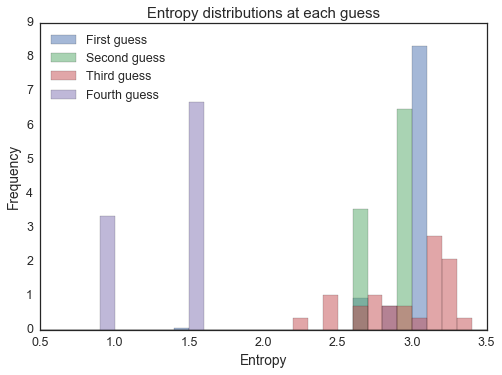
\includegraphics[width=0.6\textwidth]{img/entropy}
\caption{Entropy distributions for classic game parameters}
\label{fig:entropy}
\end{figure}

\newpage
\section{Results}

\newpage

\nocite{runarsson2010adapting}
\nocite{merelo2010finding}
\nocite{doerr2013playing}
\nocite{merelo2013improving}
\nocite{snydermastermind}
\nocite{knuth76}

\bibliographystyle{plain} 
\bibliography{project}

\end{document}
